\documentclass[11pt]{amsart}

\usepackage{amsmath,amssymb,amsthm}
\usepackage[margin=1.2in]{geometry}
\usepackage{microtype}
\usepackage{booktabs}
\usepackage{algorithm}
\usepackage{algpseudocode}
\usepackage{tikz}
\usepackage{xcolor}
\usepackage[colorlinks=true,linkcolor=blue!50!black,citecolor=blue!50!black,urlcolor=blue!50!black]{hyperref}

\newtheorem{theorem}{Theorem}[section]
\newtheorem{lemma}[theorem]{Lemma}
\newtheorem{proposition}[theorem]{Proposition}
\newtheorem{corollary}[theorem]{Corollary}
\theoremstyle{definition}
\newtheorem{definition}[theorem]{Definition}
\theoremstyle{remark}
\newtheorem{remark}[theorem]{Remark}

\newcommand{\Board}{B}
\newcommand{\Sq}{Q}


\title{A short winning rule for the square achievement game}
\author{Sean Reid}
\date{September 2026}

\begin{document}

\begin{abstract}
Two players alternately claim cells of an $n \times n$ grid, and the
first to hold the four corners of an axis-aligned square wins. In
earlier work we gave an explicit first-player strategy that wins on
every board of size at least $6$, but it consulted a lookup table of
some eight thousand forcing plans. Here we replace the table by a rule
that fits in a paragraph. The first player opens at $(2,2)$, answers
the first reply with a fixed second move, takes a completion or a
block whenever one is available, and otherwise plays the shortest
line of at most three single forcing moves followed by the arms of a
\emph{plus}: a held stone together with the four cells at a common
distance along the axes, whose arms force the opponent to block on
the diagonals and whose last arm threatens two squares at once. The
rule wins every game by the seventeenth ply, plays only $79$ distinct
lines on every board, and reads only the first player's stones, the
opponent's stones inside a $17 \times 17$ region, and one derived
cell. We verify it by exhaustive forced-tree search for boards of
size $6$ to $17$ and transport the run at $23$ to every larger board
by the simulation theorem of the earlier work. Everything is
formalized in Lean~4. The formal theorem is stronger than a bare
existence statement: it says that the tree of the rule's own moves is
a winning tree, so the theorem is about the rule and not about a
search that happened to find a win.
\end{abstract}

\maketitle

\section{Introduction}\label{sec:intro}

Two players alternately claim empty cells of an $n \times n$ grid,
the first player moving first. A player wins upon holding all four
corners of a square with horizontal and vertical sides, of any size:
the cells $(r,c)$, $(r,c+s)$, $(r+s,c)$, $(r+s,c+s)$ for some
$s \ge 1$. A full board with no such square is a draw. Erickson posed
the game \cite{erickson-pearls, opg}; it is an achievement game in
the sense of Harary \cite{harary}, played in the Maker--Maker
convention, and the general theory is in Beck \cite{beck}.

In \cite{reid-threshold} we proved that the first player has a
winning strategy if and only if $n \ge 5$. Up to $n = 4$ the game is
drawn, a fact reported earlier from computer searches by Jenrich
\cite{jenrich}; from $n = 15$ up the first player wins by strategy
stealing from the theorem of Bacher and Eliahou \cite{bacher-eliahou}
that every two-coloring of the $15 \times 15$ grid contains a
monochromatic square; and for $5 \le n \le 14$ nothing had been
published until the concurrent computer searches of Adler
\cite{adler}, which report first-player wins within $13$ plies for
$6 \le n \le 14$, with certified strategy trees for $n = 6$ and $7$.
Our proof gave one explicit strategy for every $n \ge 6$: two
reflexes, complete a square if you can and otherwise block one, over
a lookup table with $237$ branches and $8{,}135$ forcing plans, all
confined to the $6 \times 6$ corner of the board. The table was
found by search and verified by search. We asked whether there is a
winning strategy for all $n \ge 6$ that a reader can carry in their
head, with no table at all.

This paper answers that question. The strategy is a rule.

\begin{quote}
Open at $(2,2)$. Answer the first reply at $(3,2)$, except against
seven first replies next to the opening pair, for which a fixed
diagram gives the second move. If some cell completes one of your
squares, take it. Otherwise, if some cell completes an opponent
square, take it. Otherwise follow the line you chose after the second
reply: the shortest sequence of at most three single forcing moves
followed by the arms of a plus of side $1$ or $2$, preferring fewer
forcing moves, then fewer arms left to play, then the smaller plus,
then the earliest cells; and
never make a threat whose only block is the latent corner of the
opponent's two free stones.
\end{quote}

A \emph{plus} is a stone together with the four cells at a common
distance $s$ from it along the two axes, its centre and its arms.
Once the centre and one arm are held, each further arm perpendicular
to a held arm makes three corners of a square of side $s$ whose fourth
corner is the diagonal cell between them, so the opponent must block
there; the last arm is perpendicular to two held arms and threatens
two such squares at once, and no single block answers both. A
\emph{single forcing move} makes exactly one threat, which the
opponent must block; it adds a stone to the position at no cost in
tempo, and the rule uses at most three of them to prepare a plus. The
\emph{latent corner} of the opponent's two free stones is the one
cell of the $6 \times 6$ corner that completes three corners of a
square with them when such a square exists; Section~\ref{sec:defs}
recalls the definition from \cite{reid-threshold}.

\begin{theorem}\label{thm:main}
For every $n \ge 6$, the first player following the rule wins the
square achievement game on the $n \times n$ board.
\end{theorem}

Three points about the theorem. First, the rule replaces the table
entirely: no data enters the statement or the proof beyond the seven
exceptional second moves. The Lean definition of the rule is $250$
lines, most of it the search for the line, and the reader can check
by hand that it says what the paragraph above says. Second, the
theorem is about the rule's own play. The formal statement is
\[
  \texttt{plus\_wins\_with} \;:\; 6 \le n \;\longrightarrow\;
  \texttt{WinsWith}\ \texttt{plusMove}\ n\ [\,],
\]
where $\texttt{WinsWith}\ \sigma\ n\ h$ says that the game tree in
which the first player plays $\sigma$'s move at every node after the
history $h$, and the second player plays every legal reply, ends in a
first-player square on every branch. This is stronger than the
statement proved in \cite{reid-threshold}, which was that a winning
tree exists and was found by the checker; here the tree is the one
the rule plays. Third, the rule is short in play as well as in
statement. Against any opponent it wins by the seventeenth ply, on
every board; the table strategy needed $27$. On every board from $6$
to $17$ it plays the same $79$ lines, since a pair's line depends
only on its abstraction, and the lines that occur on a larger board
all occur already on $\Board_6$; each line has at most six
first-player moves after the opening pair.

The proof has the same shape as in \cite{reid-threshold}, with one
new ingredient. Boards of size $6$ to $17$ are verified by a
forced-tree checker that evaluates the rule at every node. For larger
boards a checked run on the $23 \times 23$ board, together with three
families of anchored runs, is transported to every $n \ge 17$ by the
simulation theorem of \cite{reid-threshold}. The new ingredient is an
agreement lemma: the rule reads the same move from a real history on
$\Board_n$ and from its image on the base board, in which the
opponent's far stones are replaced by fixed stand-ins, because the
stand-ins lie beyond the region the rule looks at and share the
latent corner with the stones they replace. That lemma is what turns
the simulation into a statement about the rule rather than about the
existence of a win. Section~\ref{sec:how} explains how the rule was
found in the table, and Section~\ref{sec:measure} reports what it
does on each board.

\section{Definitions}\label{sec:defs}

Cells are pairs $(r,c)$ of non-negative integers, row then column,
with row $0$ at the top and column $0$ at the left in the figures, and
$\Board_n = \{0,\dots,n-1\}^2$. The square anchored at $(r,c)$ with
side $s \ge 1$ is
$\Sq(r,c,s) = \{(r,c), (r,c+s), (r+s,c), (r+s,c+s)\}$; a set of cells
contains a square if it contains some $\Sq(r,c,s)$. We call the first
player \emph{we} and the second player \emph{the opponent}. We
\emph{threaten} at a cell $z$ if $z$ is empty and $z$ together with
three of our stones is a square; the opponent \emph{blocks} the threat
by playing $z$. A move that makes exactly one threat is \emph{forcing}:
the opponent must block or lose on the next move. A move that makes two
threats at different cells wins, since one block leaves the other. We
write $\Board_6$ for the corner region in which the rule plays and
$\Board_{17}$ for the base board whose stones it reads verbatim.
Table~\ref{tab:terms} collects the terms defined in this section.

\subsection{Pluses}

\begin{definition}[plus]\label{def:plus}
The \emph{plus} of side $s$ at the \emph{centre} $c = (r,k)$ has four
\emph{arms}, the cells $(r-s,k)$, $(r+s,k)$, $(r,k-s)$, $(r,k+s)$, and
four \emph{diagonals}, the cells $(r \pm s, k \pm s)$. Two arms are
\emph{perpendicular} if one is above or below the centre and the other
to its left or right; the diagonal between two perpendicular arms is
the cell in the row of one and the column of the other. A plus lies
in the region if its arms and diagonals do, that is, $s \le r, k$ and
$r+s, k+s \le 5$.
\end{definition}

\begin{figure}[ht]
\centering
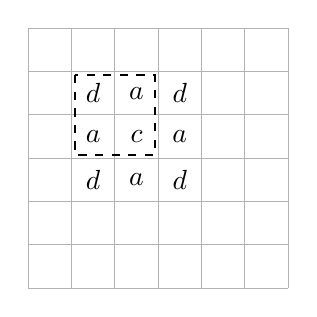
\begin{tikzpicture}[scale=0.55]
  \draw[gray!60] (0,0) grid (6,-6);
  \node at (2.5,-2.5) {$c$};
  \foreach \r/\c in {1/2, 3/2, 2/1, 2/3} \node at (\c+0.5,-\r-0.5) {$a$};
  \foreach \r/\c in {1/1, 1/3, 3/1, 3/3} \node at (\c+0.5,-\r-0.5) {$d$};
  \draw[thick,dashed] (1.08,-1.08) rectangle (2.92,-2.92);
\end{tikzpicture}
\hspace{2em}
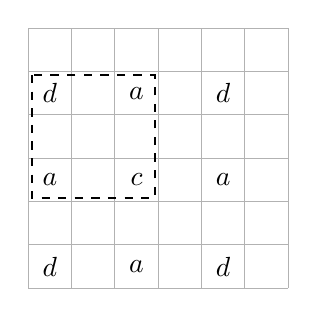
\begin{tikzpicture}[scale=0.55]
  \draw[gray!60] (0,0) grid (6,-6);
  \node at (2.5,-3.5) {$c$};
  \foreach \r/\c in {1/2, 5/2, 3/0, 3/4} \node at (\c+0.5,-\r-0.5) {$a$};
  \foreach \r/\c in {1/0, 1/4, 5/0, 5/4} \node at (\c+0.5,-\r-0.5) {$d$};
  \draw[thick,dashed] (0.08,-1.08) rectangle (2.92,-3.92);
\end{tikzpicture}
\caption{Left: the plus of side $1$ at $c = (2,2)$, with its arms $a$
and diagonals $d$. Right: the plus of side $2$ at $c = (3,2)$. In each
picture the dashed outline encloses one of the four squares of the
plus: its corners are the centre, two perpendicular arms, and the
diagonal between them. There is one such square per diagonal.}
\label{fig:anatomy}
\end{figure}

There are $16$ pluses of side $1$ in the region, with centres in
$\{1,\dots,4\}^2$, and four of side $2$, with centres in
$\{2,3\}^2$. Pluses of side $3$ do not fit. The point of the shape is
the following lemma.

\begin{lemma}[arms force]\label{lem:arms}
Suppose we hold the centre $c$ and one arm $a$ of a plus of side $s$,
and the opponent holds none of its arms and none of its diagonals.
Playing an arm $b$ perpendicular to $a$ threatens at the diagonal
between $a$ and $b$. If we hold both $a$ and the arm $a'$ opposite to
$a$, playing $b$ threatens at two cells, the diagonals between $a$ and
$b$ and between $a'$ and $b$.
\end{lemma}

\begin{proof}
Say $a = (r-s,k)$ and $b = (r,k-s)$. Then $c$, $a$, $b$ and
$d = (r-s,k-s)$ are the four corners of $\Sq(r-s,k-s,s)$, so with
$c, a, b$ held and $d$ empty we threaten at $d$. With
$a' = (r+s,k)$ also held, $c$, $a'$, $b$ and $(r+s,k-s)$ are the
corners of $\Sq(r,k-s,s)$, and $(r+s,k-s) \ne d$. The other placements
are the same up to symmetry.
\end{proof}

So from a centre and one arm, three moves win against an opponent who
has no threat of their own: the two arms perpendicular to the held arm
each force a block on a diagonal, and the opposite arm then threatens
at two diagonals at once. Blocks land on diagonals, never on arms, so
they do not get in the way. Figure~\ref{fig:basic} plays this out. The
opening $(2,2)$ and the second move $(3,2)$ are the centre and an arm
of the side-$1$ plus at $(2,2)$, and also an arm and the centre of the
side-$1$ plus at $(3,2)$; this is why the rule usually needs no
preparation at all.

\begin{figure}[ht]
\centering
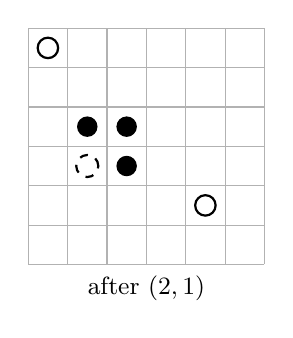
\begin{tikzpicture}[scale=0.5]
  \draw[gray!60] (0,0) grid (6,-6);
  \foreach \r/\c in {2/2, 3/2, 2/1} \fill[black] (\c+0.5,-\r-0.5) circle (0.26);
  \foreach \r/\c in {0/0, 4/4} \draw[thick] (\c+0.5,-\r-0.5) circle (0.26);
  \draw[thick,dashed] (1.5,-3.5) circle (0.28);
  \node at (3,-6.6) {\small after $(2,1)$};
\end{tikzpicture}
\hspace{1em}
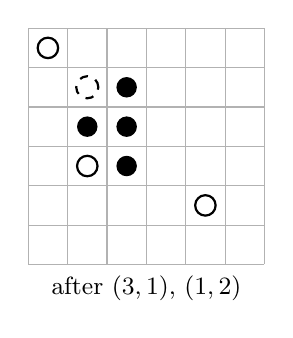
\begin{tikzpicture}[scale=0.5]
  \draw[gray!60] (0,0) grid (6,-6);
  \foreach \r/\c in {2/2, 3/2, 2/1, 1/2} \fill[black] (\c+0.5,-\r-0.5) circle (0.26);
  \foreach \r/\c in {0/0, 4/4, 3/1} \draw[thick] (\c+0.5,-\r-0.5) circle (0.26);
  \draw[thick,dashed] (1.5,-1.5) circle (0.28);
  \node at (3,-6.6) {\small after $(3,1)$, $(1,2)$};
\end{tikzpicture}
\hspace{1em}
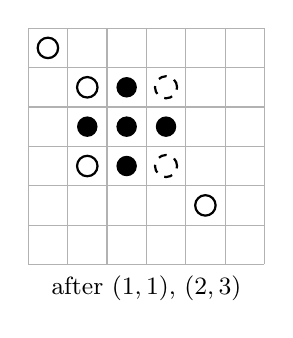
\begin{tikzpicture}[scale=0.5]
  \draw[gray!60] (0,0) grid (6,-6);
  \foreach \r/\c in {2/2, 3/2, 2/1, 1/2, 2/3} \fill[black] (\c+0.5,-\r-0.5) circle (0.26);
  \foreach \r/\c in {0/0, 4/4, 3/1, 1/1} \draw[thick] (\c+0.5,-\r-0.5) circle (0.26);
  \draw[thick,dashed] (3.5,-1.5) circle (0.28);
  \draw[thick,dashed] (3.5,-3.5) circle (0.28);
  \node at (3,-6.6) {\small after $(1,1)$, $(2,3)$};
\end{tikzpicture}
\caption{The basic line, against the replies $(0,0)$ and $(4,4)$. We
(black) hold the centre $(2,2)$ and the arm $(3,2)$. Left: the arm
$(2,1)$ threatens at the diagonal $(3,1)$, dashed. Middle: the opponent
(white) blocked there; the arm $(1,2)$ threatens at $(1,1)$. Right: the
opponent blocked again; the last arm $(2,3)$ threatens at $(1,3)$ and
$(3,3)$, and no single block answers both. We win on the ninth ply.}
\label{fig:basic}
\end{figure}

\subsection{Tempo moves and lines}

When a plus cannot be completed directly, because the opponent holds
an arm or a diagonal, or because our arms would not force, the rule
first plays a few moves that each force a block and thereby add a
stone of ours to the board.

\begin{definition}[tempo move]\label{def:tempo}
In a position where the opponent has no threat, a \emph{tempo move} is
a cell in $\Board_6$ that makes exactly one threat, such that after
the opponent blocks it the opponent still has no threat, and the block
is not the latent corner of Definition~\ref{def:latent}.
\end{definition}

A tempo move and its block add one stone to each side and return the
move to us. The opponent's new stone is where we forced it; ours is
where we chose. Figure~\ref{fig:tempo} shows two tempo moves preparing
a plus of side $2$.

\begin{figure}[ht]
\centering
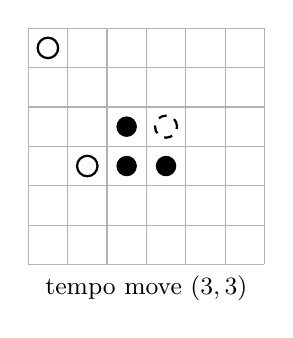
\begin{tikzpicture}[scale=0.5]
  \draw[gray!60] (0,0) grid (6,-6);
  \foreach \r/\c in {2/2, 3/2, 3/3} \fill[black] (\c+0.5,-\r-0.5) circle (0.26);
  \foreach \r/\c in {0/0, 3/1} \draw[thick] (\c+0.5,-\r-0.5) circle (0.26);
  \draw[thick,dashed] (3.5,-2.5) circle (0.28);
  \node at (3,-6.6) {\small tempo move $(3,3)$};
\end{tikzpicture}
\hspace{1em}
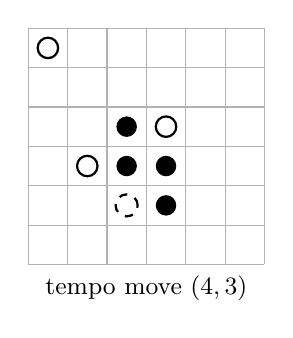
\begin{tikzpicture}[scale=0.5]
  \draw[gray!60] (0,0) grid (6,-6);
  \foreach \r/\c in {2/2, 3/2, 3/3, 4/3} \fill[black] (\c+0.5,-\r-0.5) circle (0.26);
  \foreach \r/\c in {0/0, 3/1, 2/3} \draw[thick] (\c+0.5,-\r-0.5) circle (0.26);
  \draw[thick,dashed] (2.5,-4.5) circle (0.28);
  \node at (3,-6.6) {\small tempo move $(4,3)$};
\end{tikzpicture}
\hspace{1em}
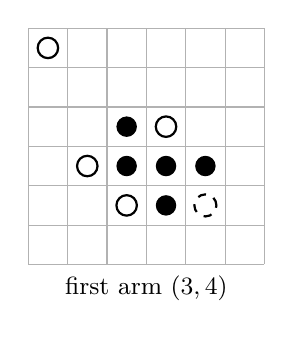
\begin{tikzpicture}[scale=0.5]
  \draw[gray!60] (0,0) grid (6,-6);
  \foreach \r/\c in {2/2, 3/2, 3/3, 4/3, 3/4} \fill[black] (\c+0.5,-\r-0.5) circle (0.26);
  \foreach \r/\c in {0/0, 3/1, 2/3, 4/2} \draw[thick] (\c+0.5,-\r-0.5) circle (0.26);
  \draw[thick,dashed] (4.5,-4.5) circle (0.28);
  \node at (3,-6.6) {\small first arm $(3,4)$};
\end{tikzpicture}
\caption{Against the replies $(0,0)$ and $(3,1)$ the side-$1$ pluses
are spoiled: $(3,1)$ is a diagonal of both. Left: the tempo move
$(3,3)$ threatens at $(2,3)$ through $\Sq(2,2,1)$. Middle: after the
block, $(4,3)$ threatens at $(4,2)$ through $\Sq(3,2,1)$. Right: after
that block, the stones $(3,3)$ and $(4,3)$ let the first arm $(3,4)$
of the side-$2$ plus at $(3,2)$ force, through the small square
$\Sq(3,3,1)$ with fourth corner $(4,4)$. From here the plus wins as
in Lemma~\ref{lem:arms}; Figure~\ref{fig:tempoend} shows the end.}
\label{fig:tempo}
\end{figure}

\begin{definition}[line, key]\label{def:line}
A \emph{line} from a position consists of some tempo moves, each
followed by its block, and then the arms of one plus in the region
that we do not yet hold, in some order, such that: each arm before the
last makes exactly one threat, whose block is not the latent corner;
the last arm played makes at least two threats; and at no point does
the opponent have a threat. The \emph{key} of a line is the triple
\[
  (\text{number of tempo moves},\ \text{number of arms to play},\
  \text{side of the plus}).
\]
The rule prefers the line with the smallest key in lexicographic
order; among lines with the same key it prefers the smaller centre in
cell order, and among those the one its search generates first.
\end{definition}

The number of arms to play is three when we hold the centre and one
arm, as in the basic line, and fewer if earlier moves have put us on
more arms. The rule searches for lines with at most three tempo moves.
Whether a line exists, and which one is preferred, depends only on the
abstract position defined next.

\subsection{Far stones and the latent corner}

\begin{definition}[latent corner, abstraction]\label{def:latent}
Two cells $x, y$ have a \emph{latent square} with corner $b$ if
$b \in \Board_6$, the three cells $b, x, y$ are corners of one square,
and that square is not contained in $\Board_{17}$; $b$ is the
\emph{latent corner} of the pair. The \emph{abstraction} of a position
in which we have moved at least twice consists of our stones, the
opponent's stones inside $\Board_{17}$, and the latent corner of the
opponent's first two stones, if they have one.
\end{definition}

\begin{figure}[ht]
\centering
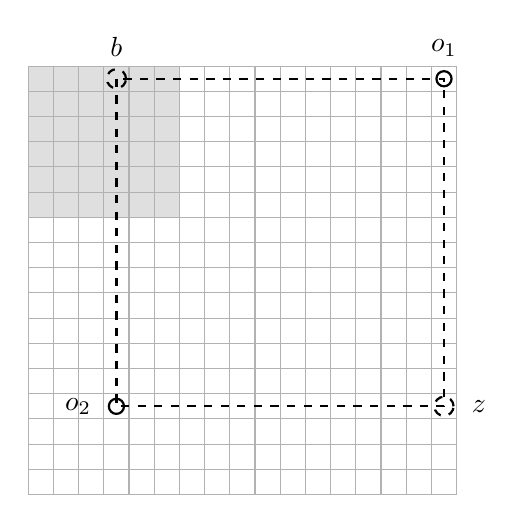
\begin{tikzpicture}[scale=0.32]
  \fill[gray!25] (0,0) rectangle (6,-6);
  \draw[gray!60] (0,0) grid (17,-17);
  \draw[thick,dashed] (3.5,-0.5) rectangle (16.5,-13.5);
  \foreach \r/\c in {0/16, 13/3}
    \draw[thick] (\c+0.5,-\r-0.5) circle (0.3);
  \draw[thick,dashed] (3.5,-0.5) circle (0.38);
  \draw[thick,dashed] (16.5,-13.5) circle (0.38);
  \node[above=1pt] at (3.5,-0.1) {$b$};
  \node[above=1pt] at (16.5,-0.1) {$o_1$};
  \node[left=2pt] at (3.1,-13.5) {$o_2$};
  \node[right=2pt] at (17.0,-13.5) {$z$};
\end{tikzpicture}
\caption{A latent square, drawn on $\Board_{17}$. The opponent's free
replies $o_1 = (0,16)$ and $o_2 = (13,3)$ are two corners of the dashed
square, whose third corner $b = (0,3)$ lies in the region (shaded)
and whose fourth corner $z = (13,16)$ lies just outside $\Board_{17}$.
The rule never threatens at $b$: if the opponent had to block there
they would threaten at $z$.}
\label{fig:latent}
\end{figure}

Two facts from \cite[Section~6]{reid-threshold} explain the
abstraction. First, two stones in $\Board_6$ lie in a common square
only if that square lies in $\Board_{12}$. In a position the rule
reaches, the opponent's stones are the two free replies and forced
blocks, and the blocks lie in $\Board_6$. So a stone beyond
$\Board_{17}$ shares no square with two blocks, and a square through
such a stone and one block has both free replies as its other corners:
it is a latent square. Second, a pair of cells has at most one latent
corner, and only pairs whose members both have a coordinate at least
$12$ have one. Hence the stones the rule cannot see, the opponent's
stones beyond $\Board_{17}$, can affect the game only through the
latent corner, and the rule records exactly that cell. The clause of
Definition~\ref{def:tempo} that keeps blocks off the latent corner is
what prevents a far pair from ever coming into play: if the opponent
were forced to block on $b$ in Figure~\ref{fig:latent}, they would
hold three corners of the latent square and threaten at $z$, and we
would have to answer instead of continuing our line.

\begin{table}[ht]
\centering
\begin{tabular}{lp{0.68\textwidth}}
\toprule
term & meaning \\
\midrule
threat & an empty cell that completes one of our squares \\
block & the opponent's move on a threat cell \\
forcing move & a move that makes exactly one threat \\
plus & a centre with four arms at distance $s$ along the axes \\
arm, diagonal & a cell of the plus on an axis; a cell of the plus off the axes \\
tempo move & a forcing move in $\Board_6$ whose block leaves the opponent without a threat and misses the latent corner \\
line & tempo moves, then the arms of one plus, the last arm making two threats \\
key & (tempo moves, arms to play, side); smaller is preferred \\
latent corner & the region cell completing three corners of a square with the two free replies, when the square leaves $\Board_{17}$ \\
abstraction & our stones, the opponent's stones in $\Board_{17}$, the latent corner \\
\bottomrule
\end{tabular}
\medskip
\caption{The terms of the rule.}
\label{tab:terms}
\end{table}

\section{The rule}\label{sec:rule}

Algorithms~\ref{alg:move} and~\ref{alg:line} state the rule as it is
defined in the formal development. The first is the move function; the
second is the search it calls once, after the second reply, to choose
the line. The second move against a first reply $o_1$ is $(3,2)$
unless $o_1$ is one of seven cells, for which Figure~\ref{fig:second}
gives the move.

\begin{algorithm}[ht]
\caption{The move function.}\label{alg:move}
\begin{algorithmic}[1]
\If{some cell completes one of our squares}
  \State play the least such cell
\ElsIf{some cell completes an opponent square}
  \State play the least such cell
\ElsIf{we have not yet moved}
  \State play $(2,2)$
\ElsIf{we do not yet hold the second move for the first reply $o_1$}
  \State play it
\Else
  \State let $L$ be the line of Algorithm~\ref{alg:line} for the
    abstraction of the position after the second reply
  \State play the first cell of $L$ that we do not hold
\EndIf
\end{algorithmic}
\end{algorithm}

\begin{algorithm}[ht]
\caption{The line search, from an abstract position $A$.}\label{alg:line}
\begin{algorithmic}[1]
\State $F \gets \{(A, \text{empty prefix})\}$
\For{$d = 0, 1, 2, 3$}
  \ForAll{$(B, p) \in F$ in order, if the opponent has no threat in $B$}
    \ForAll{pluses in the region whose centre we hold in $B$, side $1$ then $2$}
      \State the arms to play are those we do not hold; skip the plus if the opponent holds one
      \State try the orders of these arms; keep the first that wins by force (Definition~\ref{def:line})
    \EndFor
    \State record the best plus found from $B$, by (arms to play, side, centre), behind $p$
  \EndFor
  \If{some plus was recorded} \Return the recorded line with the smallest key \EndIf
  \State $F \gets \{(B', p\,m) : (B, p) \in F,\ m \text{ a tempo move in } B,\ B' = B \text{ after } m \text{ and its block}\}$
\EndFor
\State \Return no line
\end{algorithmic}
\end{algorithm}

The loop over $d$ is what makes fewer tempo moves come first: all
lines with $d$ tempo moves are examined before any with $d+1$. Within
one value of $d$ the key compares the arms to play, then the side,
then the centre. The order in which tempo moves and arm orders are
tried is fixed, cell order for tempo moves and a fixed enumeration of
permutations for arms, so that two implementations of the rule choose
the same line; the Lean definition and the Python twin are compared on
this.

\begin{figure}[ht]
\centering
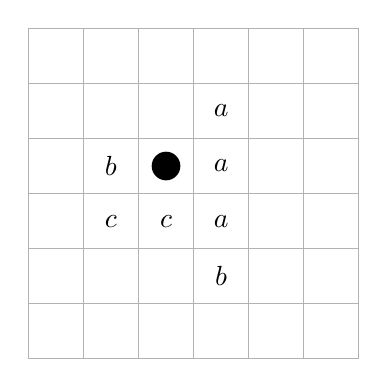
\begin{tikzpicture}[scale=0.7]
  \draw[gray!60] (0,0) grid (6,-6);
  \fill[black] (2.5,-2.5) circle (0.26);
  \foreach \r/\c/\t in {1/3/a, 2/3/a, 3/3/a, 2/1/b, 4/3/b, 3/1/c, 3/2/c}
    \node at (\c+0.5,-\r-0.5) {$\t$};
\end{tikzpicture}
\caption{The second move. The black stone is the opening. Against a
first reply on a cell marked $a$ the second move is $(2,1)$; on a cell
marked $b$ it is $(2,3)$; on a cell marked $c$ it is $(1,2)$. Against
every other first reply, on this board or beyond it, the second move
is $(3,2)$. The cell $(2,3)$ is marked $a$ and $(2,1)$ is marked $b$:
when the reply takes one of the natural second moves, the rule takes
the other.}
\label{fig:second}
\end{figure}

The exceptions are exactly the first replies from which the default
second move fails. The choice of $(3,2)$ and the order in which
alternatives are tried, $(3,2)$, $(2,3)$, $(2,1)$, $(1,2)$, came from
search: for each first reply on $\Board_6$ the second move is the
first cell in that order against which the rest of the rule beats
every second reply. All seven exceptions lie within one king's move of
the opening or of $(3,2)$, and one of them is $(3,2)$ itself; the
farthest, $(4,3)$, is a diagonal of the side-$1$ plus at $(3,2)$, the
cell on which the default line would need the opponent to block.

\subsection{Two games}

Table~\ref{tab:games} lists two complete games against an opponent
who always blocks, the shortest kind of line and the longest. In the
first the replies $(0,0)$ and $(4,4)$ are far from the opening pair
and the basic line of Figure~\ref{fig:basic} wins at once: no tempo
moves, three arms, side $1$, key $(0,3,1)$. In the second the reply
$(3,1)$ sits on a diagonal of both side-$1$ pluses, and the rule
finds nothing with fewer than two tempo moves; its line has key
$(2,4,2)$, the side-$2$ plus at $(3,2)$ with all four arms to play,
prepared by the two tempo moves of Figure~\ref{fig:tempo}. This is the
longest game the rule ever plays: the win comes on the seventeenth
ply, on every board.

\begin{table}[ht]
\centering
\small
\begin{tabular}{rllp{0.5\textwidth}}
\toprule
ply & we & opponent & what the move does \\
\midrule
1, 2 & $(2,2)$ & $(0,0)$ & opening; free reply \\
3, 4 & $(3,2)$ & $(4,4)$ & second move; free reply \\
5, 6 & $(2,1)$ & $(3,1)$ & arm; threat at $(3,1)$ through $\Sq(2,1,1)$, blocked \\
7, 8 & $(1,2)$ & $(1,1)$ & arm; threat at $(1,1)$ through $\Sq(1,1,1)$, blocked \\
9 & $(2,3)$ & & arm; threats at $(1,3)$ and $(3,3)$; wins \\
\midrule
1, 2 & $(2,2)$ & $(0,0)$ & opening; free reply \\
3, 4 & $(3,2)$ & $(3,1)$ & second move; free reply on a diagonal \\
5, 6 & $(3,3)$ & $(2,3)$ & tempo move; threat at $(2,3)$ through $\Sq(2,2,1)$ \\
7, 8 & $(4,3)$ & $(4,2)$ & tempo move; threat at $(4,2)$ through $\Sq(3,2,1)$ \\
9, 10 & $(3,4)$ & $(4,4)$ & arm; threat at $(4,4)$ through $\Sq(3,3,1)$ \\
11, 12 & $(1,2)$ & $(1,4)$ & arm; threat at $(1,4)$ through $\Sq(1,2,2)$ \\
13, 14 & $(5,2)$ & $(5,4)$ & arm; threat at $(5,4)$ through $\Sq(3,2,2)$ \\
15, 16 & $(3,0)$ & $(1,0)$ & arm; threats at $(1,0)$ and $(5,0)$; one is blocked \\
17 & $(5,0)$ & & completes $\Sq(3,0,2)$; wins \\
\bottomrule
\end{tabular}
\medskip
\caption{Two games against an opponent who always blocks. Above, the
basic line; below, the longest line. In the second game the arms of
the side-$2$ plus at $(3,2)$ are $(1,2)$, $(5,2)$, $(3,0)$, $(3,4)$;
the first of them is forced through a small square with the tempo
stones, the next two through side-$2$ squares with the centre and the
arm $(3,4)$, and the last threatens at two diagonals.}
\label{tab:games}
\end{table}

\begin{figure}[ht]
\centering
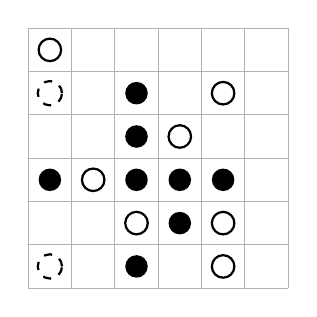
\begin{tikzpicture}[scale=0.55]
  \draw[gray!60] (0,0) grid (6,-6);
  \foreach \r/\c in {2/2, 3/2, 3/3, 4/3, 3/4, 1/2, 5/2, 3/0}
    \fill[black] (\c+0.5,-\r-0.5) circle (0.26);
  \foreach \r/\c in {0/0, 3/1, 2/3, 4/2, 4/4, 1/4, 5/4}
    \draw[thick] (\c+0.5,-\r-0.5) circle (0.26);
  \draw[thick,dashed] (0.5,-1.5) circle (0.28);
  \draw[thick,dashed] (0.5,-5.5) circle (0.28);
\end{tikzpicture}
\caption{The position after the fifteenth ply of the second game in
Table~\ref{tab:games}. The side-$2$ plus at $(3,2)$ is complete except
for the opponent's blocks on its diagonals $(1,4)$ and $(5,4)$; the
last arm $(3,0)$ threatens at the other two diagonals, dashed.}
\label{fig:tempoend}
\end{figure}

The line is chosen once, after the second reply, and followed. The
opponent's blocks are forced, so in the tree the checker verifies
every later position on a branch is determined by the line, and our
stones at any point are the opening pair and a prefix of the line. A
rule that recomputed the line at every move would also be a rule of
this kind; we fixed the committed version because it makes the
verified tree a function of the reply pair, which is what the argument
of Section~\ref{sec:uniform} needs.

The rule is quick to evaluate. The Lean definition, run compiled,
finds the line from an abstract position in about $80$ microseconds,
and the Python twin in a quarter of a millisecond. The search examines
at most three levels of tempo moves, each with at most $36$
candidates, and at each position at most $20$ pluses with at most
$24$ arm orders each.

\section{How the rule was found}\label{sec:how}

The table of \cite{reid-threshold} was generated by search on
$\Board_{15}$: for each reply pair a forcing plan was found by
depth-first search over forcing moves, with a preference for short
plans. It had $8{,}135$ plan entries and $248$ latent entries,
$8{,}383$ in all, but only $186$ distinct plans, and $8{,}354$ of the
entries begin with $(2,1)$ or $(2,3)$, an arm of the side-$1$ plus at
$(2,2)$ or at $(3,2)$. The shortest plans are that plus: two plans of
three moves, used in $157$ entries, play its three free arms in some
order and win on the ninth ply. The longer plans, which are the bulk
of the table, mostly continue from the first arm into a ladder, a run
of side-$1$ threats climbing a column, such as $(2,1)$, $(1,1)$,
$(1,0)$, $(0,0)$, and then finish elsewhere. Replaying the long plans
in the positions where they are used, the moves that make them long
do one of two things: they force a block in order to place a stone
that a later square needs, or they are the arms of a plus of side $2$
centred at $(3,2)$, forced one at a time, with the last arm making the
double threat. That is the observation behind the rule: a plan is a
plus, possibly prepared by a few forcing moves.

The first attempt at a rule did not use shapes. It scored moves by
mobility, the number of threats the first player could make next, and
played the highest score. It fails: on $\Board_6$ it leaves $31$
reply pairs without a win, all with both replies near the opening,
where the opponent's stones interfere with any single square and the
right move is a preparation whose value a one-move lookahead does not
see. The plus rule replaces the score by a target. It asks which plus
can be completed by force, allowing a few tempo moves first, and the
order of preference, fewer tempo moves, then a smaller plus, was
chosen to make the lines short; the ordering is also what makes the
choice of a line unambiguous, which the formal development needs.

Two constants were settled by trying alternatives. A depth of three
tempo moves is necessary: with two, $25$ reply pairs on $\Board_6$
have no line. It is also sufficient on every board up to $17$, and a
fourth tempo move is never used, though the rule would allow it if we
raised the bound. Pluses of side $3$ do not fit in the region, so
sides $1$ and $2$ are all there is. Finally the base board of the
abstraction was set at $17$ after a smaller choice failed: reading
only the opponent's stones inside $\Board_{12}$ loses on
$\Board_{13}$ and above, because a stone with a coordinate between
$12$ and $16$ can complete a square with one stone of the region and
one near stone, a square of side at least $7$ that lies inside
$\Board_{17}$. The base $17$ is also the least board on which the
dichotomy of Definition~\ref{def:latent} holds \cite{reid-threshold},
so the two uses of the constant agree.

Compiling the rule into a table of the old format gives $237$
branches with $2{,}330$ plan entries and $140$ latent entries, against
$8{,}135$ and $248$ before, and the same $79$ distinct lines that
Section~\ref{sec:measure} counts directly. Replaying the compiled
table and the rule against each other, they agree move for move on
every branch.

\section{Verification}\label{sec:verify}

Fix a strategy $\sigma$ and a board size $n$. The \emph{forced tree}
of $\sigma$ on $\Board_n$ is the game tree in which the first player
plays $\sigma$'s move, the second player's replies range over all
empty cells at the first two levels, and below every later node only
over the cells that block a threat of the move just played. The
checker of \cite{reid-threshold} walked this tree for the table
strategy under guards: past the second reply, every move of $\sigma$
wins outright or leaves a threat, every non-winning move and every
threat cell lies in $\Board_6$, and no empty cell completes an
opponent square. Its soundness theorem said that if every branch ends
in a first-player square then the first player can win on
$\Board_n$: a reply that blocks nothing leaves a threat standing, and
the strategy completes it next move, so every reply the tree omits
loses in two plies.

Here the checker is the same, evaluated on the rule instead of the
table, and its soundness theorem is stronger.

\begin{proposition}\label{prop:forced}
Let $\sigma$ be a strategy that, whenever the first player's stones
lie in $\Board_6$ and some cell completes one of their squares, plays
such a cell. If the forced tree of $\sigma$ on $\Board_n$ passes the
guards and every branch ends in a first-player square, then the tree
of $\sigma$'s own moves against every reply is winning:
$\texttt{WinsWith}\ \sigma\ n\ [\,]$.
\end{proposition}

The hypothesis on $\sigma$ is what the two-ply argument needs: against
a reply that blocks nothing, the winning tree must play the
completion, and if the tree is to be $\sigma$'s own tree, $\sigma$
must be the one to play it. The rule satisfies the hypothesis by its
first clause, once one knows that the executable scan it uses to find
completions agrees with the checker's; that is the content of the
Lean file \texttt{Plus/Threats.lean}, and the rule's part of the
proposition is the theorem \texttt{plusMove\_takesWins}. The
proposition itself is \texttt{checkForcedS\_winsWith}. The table
strategy of \cite{reid-threshold} also satisfies the hypothesis, so
its theorem is strengthened as well, though we do not use that here.

The rule passes the forced tree on every board from $6$ to $17$.
Table~\ref{tab:runs} gives the number of reply pairs at the root of
each tree and the wall-clock time of the compiled Lean checker.

\begin{table}[ht]
\centering
\begin{tabular}{rrrcrrr}
\toprule
$n$ & pairs & time (s) & & $n$ & pairs & time (s) \\
\midrule
6 & 1{,}155 & 0.9 & & 12 & 20{,}163 & 10 \\
7 & 2{,}208 & 1.2 & & 13 & 27{,}888 & 16 \\
8 & 3{,}843 & 1.9 & & 14 & 37{,}635 & 24 \\
9 & 6{,}240 & 2.9 & & 15 & 49{,}728 & 36 \\
10 & 9{,}603 & 4.4 & & 16 & 64{,}515 & 51 \\
11 & 14{,}160 & 6.8 & & 17 & 82{,}368 & 75 \\
\bottomrule
\end{tabular}
\medskip
\caption{Forced-tree runs of the rule: the number of reply pairs
$(o_1, o_2)$ at the root and the wall-clock time of the compiled Lean
checker on a laptop. The run on the anchor board $\Board_{23}$, with
$277{,}728$ pairs, takes $497$ seconds, and the three anchored
families of Section~\ref{sec:uniform} together take $0.35$ seconds.
Each run is discharged by native evaluation inside the build of the
development.}
\label{tab:runs}
\end{table}

As in \cite{reid-threshold} the search exists three times: a Python
twin of the rule used while finding it, the Lean definition, and the
compiled Lean checker that the proof cites. The Python twin and the
Lean rule are compared line for line on sample positions in the test
suite, and the Python verifier, which walks the full tree rather than
the forced skeleton, confirms the win on $\Board_6$ with the same
longest game.

\section{Every larger board}\label{sec:uniform}

\begin{theorem}\label{thm:uniform}
For every $n \ge 17$ the first player following the rule wins on
$\Board_n$.
\end{theorem}

The proof transports a checked run to every larger board, as in
\cite[Section~6]{reid-threshold}. We recall the mechanism and then
explain what is new. In a position the forced run can reach, the
opponent's lasting stones are the two free replies and forced blocks
in $\Board_6$. Replies inside the base board $\Board_{17}$ are read
verbatim. A reply beyond it is replaced, for the purpose of the base
run, by a stand-in: a fixed cell beyond $\Board_{17}$ when the pair
has no latent corner, and an anchor cell realizing the same latent
corner when it has one. The base run is on $\Board_{23}$, the least
board holding every anchor. Safety at every node reduces to the
dichotomy of Definition~\ref{def:latent}: an opponent square is
either inside $\Board_{17}$, and excluded by the base run, or latent,
with a corner the rule never surrenders. The far pairs with a latent
corner are covered by three families of anchored runs, one per
placement of the pair on the corners of a latent square, over all
coordinates; there are $176$ anchored positions, each a run of the
checker with the latent corner as an additional guard.

The formal simulation theorem takes a strategy $\sigma$ as a
parameter. Its conclusion is now $\texttt{WinsWith}\ \sigma\ n\ h$
for the real history $h$, and it has two hypotheses about $\sigma$
that the table version did not need. One is the hypothesis of
Proposition~\ref{prop:forced}, that $\sigma$ takes its completions.
The other is agreement:
\[
  \sigma\,(\text{real history}) \;=\; \sigma\,(\text{base history})
\]
at every node, where the base history is the real one with the two
replies replaced by their stand-ins. For the rule this is a
consequence of what it reads. The stand-ins and anchors lie beyond
$\Board_{17}$, as do the stones they replace, so both drop out of the
abstraction; a reply inside $\Board_{17}$ is its own stand-in; and the
stand-ins are chosen with the same latent corner as the real pair,
which for the anchors is part of what the anchored run checks and for
the keyless stand-ins is a short computation. So the abstractions
agree, and the rule's move is a function of the abstraction and of
the first reply's second move, which agrees too because every reply
beyond $\Board_6$ has the default second move. This is the theorem
\texttt{plusMove\_agree} in \texttt{Plus/Agreement.lean}. The table
strategy needed no such lemma because its lookups were designed
around the stand-ins; the rule needs it because nothing in its
definition mentions them.

\begin{remark}
The base board $23$, the stand-ins $(22,22)$ and $(22,21)$, and the
anchor cells at coordinates $17$ and above are choices of the proof,
not of the rule. Any board of size at least $17$ that holds the
anchors would do. The rule itself has two constants, the region $6$
and the base $17$.
\end{remark}

Theorem~\ref{thm:main} follows from the runs of
Table~\ref{tab:runs} for $6 \le n \le 17$ and from
Theorem~\ref{thm:uniform} for $n \ge 17$. The formal assembly is
\texttt{plus\_wins\_with}, with \texttt{plus\_wins} the corollary in
the form of \cite{reid-threshold}, a first-player win from the empty
board with the moves forgotten.

\section{Formalization}\label{sec:lean}

The development of \cite{reid-threshold} defines the game and the
predicate \texttt{P1CanWin}: the first player can win from a
position if some legal move completes one of their squares, or some
legal move admits a reply and every reply completes nothing and leads
to a position from which the first player can win. A derivation is a
strategy tree. Two additions carry this paper.

The first is the predicate \texttt{WinsWith}. For a strategy
$\sigma$, a board size $n$, and a history $h$ with the first player
to move, $\texttt{WinsWith}\ \sigma\ n\ h$ holds if $\sigma$'s move
at $h$ is legal and completes a square, or is legal, admits a reply,
and every reply completes nothing and leads to a history at which
\texttt{WinsWith} holds again. It has the constructors of
\texttt{P1CanWin} with one extra premise on each, that the move is
the one $\sigma$ returns, and it implies \texttt{P1CanWin} by
forgetting that premise (\texttt{WinsWith.p1CanWin}). The distinction
matters for what the theorem says. A checker that searched for a win
and found one proves \texttt{P1CanWin}. A checker that plays $\sigma$
at every node and finds that every branch wins proves
\texttt{WinsWith} for $\sigma$ only if the soundness proof never has
to invent a move; the one place it did, the two-ply win against a
reply that blocks nothing, is where Proposition~\ref{prop:forced}
needs its hypothesis.

The second is the rule as a Lean definition, \texttt{plusMove}, with
the same type as the table strategy: a function from the list of
squares of the board and the history to a move. The checker and the
simulation theorem were already generic in the strategy, so no
checker was written for this paper; the rule is passed where the
table was. The library \texttt{Plus} has six files:
\texttt{Rule.lean} defines the rule ($250$ lines), \texttt{Threats.lean}
proves that its threat scan agrees with the checker's ($190$ lines),
\texttt{Agreement.lean} proves the agreement lemma ($110$ lines),
\texttt{Anchors.lean} defines the anchored runs ($65$ lines),
\texttt{Uniform.lean} is the case analysis over the reply pairs that
assembles Theorem~\ref{thm:uniform} from the simulation
($530$ lines), and \texttt{Results.lean} evaluates the certificates
and states the theorems ($70$ lines). No table appears anywhere.

The certificates are discharged by native evaluation
(\texttt{native\_decide}), as in \cite{reid-threshold}: one for the
runs at sizes $6$ to $16$, one for size $17$, one for the anchor board,
and one for each of the three anchored families. The axioms of
\texttt{plus\_wins\_with} are \texttt{propext},
\texttt{Classical.choice}, \texttt{Quot.sound}, and these six
evaluation axioms. The kernel checks every proof except the
evaluations, which are performed by the Lean compiler and runtime.
The library builds in about thirteen minutes on a laptop, almost all
of it the evaluations.

\section{Measurements}\label{sec:measure}

For each board size from $6$ to $17$ we ran the Python twin over
every reply pair and recorded the line the rule commits to, the
number of tempo moves in front of the plus, and the ply at which the
win comes against an opponent who blocks. Table~\ref{tab:lines}
summarizes the result, which is the same on every board.

\begin{table}[ht]
\centering
\begin{tabular}{lr}
\toprule
distinct lines & 79 \\
lines with $0$, $1$, $2$, $3$ tempo moves (pairs on $\Board_6$)
  & 985, 91, 54, 25 \\
pairs using a plus of side $1$, side $2$ (on $\Board_6$) & 985, 170 \\
longest line, in first-player moves after the opening pair & 6 \\
latest winning ply & 17 \\
\bottomrule
\end{tabular}
\medskip
\caption{The rule's lines. The counts of distinct lines, the longest
line, and the latest winning ply are the same on every board from
$6$ to $17$. The numbers of pairs using two or three tempo moves,
$54$ and $25$, are also the same on every board, since such pairs
have both replies in $\Board_6$; the pairs using no tempo move grow
with the board.}
\label{tab:lines}
\end{table}

Three observations. First, the set of lines does not depend on the
board: a pair's line depends only on its abstraction, and comparing
the sets of lines directly, every board from $6$ to $17$ plays exactly
the $79$ lines that occur on $\Board_6$. Second, most pairs need no preparation: on
$\Board_{17}$, $81{,}186$ of the $82{,}368$ pairs are won by a
side-$1$ plus with no tempo move, and the other $1{,}182$ by a
side-$2$ plus behind one to three tempo moves. Only $79$ pairs on any
board, all with both replies in $\Board_6$, need two or three tempo
moves. Third, the rule is
faster than the table without being designed for speed. The latest
winning ply is $17$ against $27$ for the table of
\cite{reid-threshold}, in the same measure, the ply of the winning
move against the most stubborn opponent. The searches of Adler
\cite{adler} report wins by ply $13$ for $6 \le n \le 14$, so the
rule is not optimal in length; Section~\ref{sec:open} returns to
this.

\section{Reproducibility}\label{sec:repro}

The supplementary material contains the Lean development. In its
namespace \texttt{Plus}, Theorem~\ref{thm:main} is
\texttt{plus\_wins\_with} and Theorem~\ref{thm:uniform} is
\texttt{plus\_wins\_with\_of\_seventeen\_le};
Proposition~\ref{prop:forced} is \texttt{checkForcedS\_winsWith},
and the supporting layer is named above. The build evaluates every
certificate. Two commands of the checker executable reproduce the runs
of Table~\ref{tab:runs}:
\begin{quote}
\texttt{lake exe checker $n$ plus} \\
\texttt{lake exe checker plus anchors}
\end{quote}
The first runs the forced checker on the rule for one board and
reports its time; the second runs the three anchored families. The
Python twin of the rule lives in the pipeline as
\texttt{squares/plus}, with two commands:
\begin{quote}
\texttt{python -m squares.plus.sweep $n$} \\
\texttt{python -m squares.plus.measure}
\end{quote}
The first sweeps every reply pair on $\Board_n$ and replays the
anchored positions; the second produces Table~\ref{tab:lines}. The
test suite checks the twin against the Lean rule on sample positions
and runs the full verifier on $\Board_6$.

\section{Open questions}\label{sec:open}

The rule wins by ply $17$; Adler's searches \cite{adler} find wins by
ply $13$ on each board from $6$ to $14$, one search per board. Is
there a rule of comparable length that wins by ply $13$ on every
board, and what is the least ply by which the first player can force
a win on $\Board_n$? The rule's ordering prefers fewer tempo moves
and then smaller pluses; other orderings, or other target shapes,
might shorten the longest games at the cost of a longer statement.

The second move has seven exceptions. Is there an opening pair, or an
opening move with a fixed second move, from which a rule of this kind
wins with no exceptions? The search that fixed the second move tried
the four neighbours of the opening in one order; we did not search
over openings.

The rule does not apply to $\Board_5$. There the table of
\cite{reid-threshold} needed quiet moves, non-threatening moves
followed by a case split on the reply, because from twenty reply
pairs no purely forcing continuation wins. A short rule for
$\Board_5$, with quiet moves allowed, is open.

Finally, the constants. The region $6$ cannot shrink for a purely
forcing strategy from $(2,2)$ \cite{reid-threshold}. The base $17$ is
least for the dichotomy of latent squares, and the abstraction that
reads $\Board_{17}$ verbatim is what the proof needs; whether a rule
can read less, for instance only the opponent's stones inside
$\Board_6$ together with a summary of the rest, is open.

\section*{Acknowledgements}

I thank Nicholas Tan for many games and for productive discussions
that shaped the strategy presented here.

\bibliographystyle{amsplain}
\bibliography{../shared/refs}

\end{document}
